\documentclass[tikz,border=2mm]{standalone}
\usepackage{tikz}
\begin{document}
   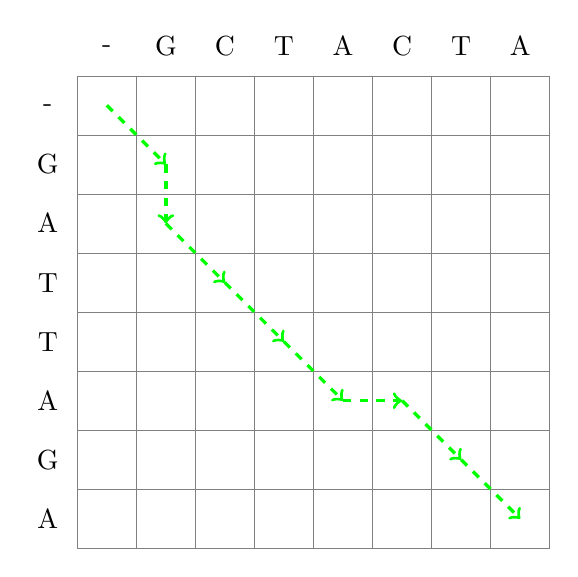
\begin{tikzpicture}[set style={{help lines}+=[dashed]}, xscale=0.75, yscale=0.75]
   % Grid
   \draw[step=1cm,gray,very thin] (0,-1) grid (8,7);
   
   % Labels for GATTAGA
   \node at (-0.5, 6.5) {-};
   \node at (-0.5, 5.5) {G};
   \node at (-0.5, 4.5) {A};
   \node at (-0.5, 3.5) {T};
   \node at (-0.5, 2.5) {T};
   \node at (-0.5, 1.5) {A};
   \node at (-0.5, 0.5) {G};
   \node at (-0.5, -0.5) {A};
   
   % Labels for GCTACTA
   \node at (0.5, 7.5) {-};
   \node at (1.5, 7.5) {G};
   \node at (2.5, 7.5) {C};
   \node at (3.5, 7.5) {T};
   \node at (4.5, 7.5) {A};
   \node at (5.5, 7.5) {C};
   \node at (6.5, 7.5) {T};
   \node at (7.5, 7.5) {A};
   
   % First alignment
   \draw[green, very thick, dashed, ->] (0.5,6.5) -- (1.5,5.5);  % G -> G
   \draw[green, very thick, dashed, ->] (1.5,5.5) -- (1.5,4.5);  % Gap 
   \draw[green, very thick, dashed, ->] (1.5,4.5) -- (2.5,3.5);  % T -> C
   \draw[green, very thick, dashed, ->] (2.5,3.5) -- (3.5,2.5);  % T -> T
   \draw[green, very thick, dashed, ->] (3.5,2.5) -- (4.5,1.5);  % A -> A
   \draw[green, very thick, dashed, ->] (4.5,1.5) -- (5.5,1.5);  % Insert
   \draw[green, very thick, dashed, ->] (5.5,1.5) -- (6.5,0.5);  % T -> G
   \draw[green, very thick, dashed, ->] (6.5,0.5) -- (7.5,-0.5);  % A -> A
   
   
   \end{tikzpicture}
\end{document}
